%\newpage
%\section{Revisão da Teoria}
%
%\subsection{Modulação ASK}
%
%A modulação ASK ("\emph{Amplitude Shift Keying}") é uma maneira bem simples de modulação digital. Essa técnica consiste em transmitir dados através da variação da amplitude da tensão de um sinal, ou seja, a informação a ser transmitida é inserida na amplitude de uma sequência de pulsos elétricos, como mostra a figura \ref{fig:mask}. 
%
%\begin{figure}[H]
%    \centering
%    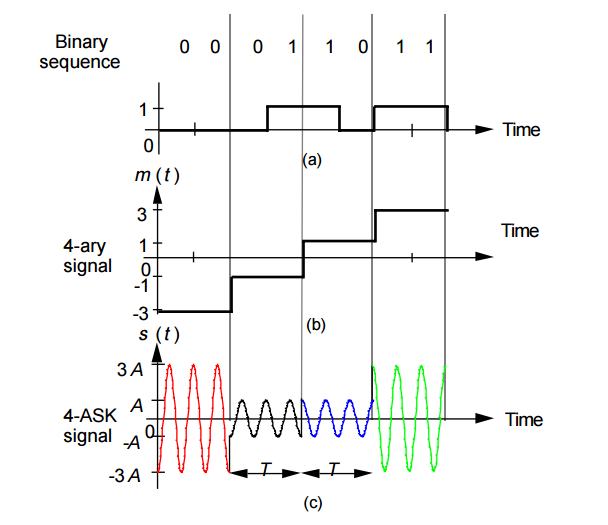
\includegraphics[scale=0.7]{mask}
%    \caption{Modulação 4-ASK de um sinal de dados.}
%    \label{fig:mask}
%\end{figure}
%
%\subsubsection{Modulador ASK}
%O modulador ASK é de fácil implementação, pois consiste em um multiplicador, o qual multiplica a portadora, de frequência $f_c$, pelo sinal digital, como pode ser visto na figura \ref{fig:modASK}.
%
%\begin{figure}[H]
%    \centering
%    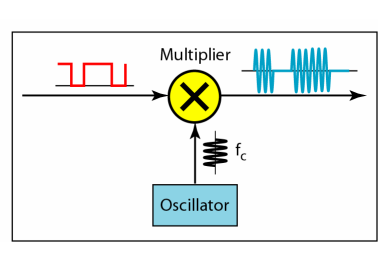
\includegraphics[scale=0.7]{modASK}
%    \caption{Modulador ASK.}
%    \label{fig:modASK}
%\end{figure}
%
%Para o M-ASK, é necessário codificar os dados de entrada antes de aplicar a modulação (vide figura \ref{fig:mask} (b)), fazendo com que cada conjunto de bits se torne um nível de tensão distinto.
% 
%\subsection{Modulação FSK}
%
%A modulação FSK ("\emph{Frequency Shift Keying}") é uma técnica de modulação que consiste em variar a frequência da portadora em função do sinal modulante, no caso o sinal digital a ser transmitido.
%Pode-se considerar que este tipo de modulação é equivalente a modulação FM analógica.
%
%A amplitude da onda portadora modulada é mantida constante durante todo o processo de modulação, quando o sinal digital apresenta nível lógico "1" a frequência da portadora é alterada para posteriormente ser detectada no processo de demodulação.
%A frequência resultante transmitida será a frequência da onda portadora $f_c$ diminuida de uma frequência de desvio $f_d$.
%Ou seja
%\begin{equation}
%f_r = f_c - f_d
%\end{equation}
%
%Para a ocorrência de um nível lógico "0", a frequência resultante será a frequência da portadora mais a frequência de desvio.
%\begin{equation}
%f_r = f_c + f_d
%\end{equation}
%
%\begin{figure}[H]
%    \centering
%    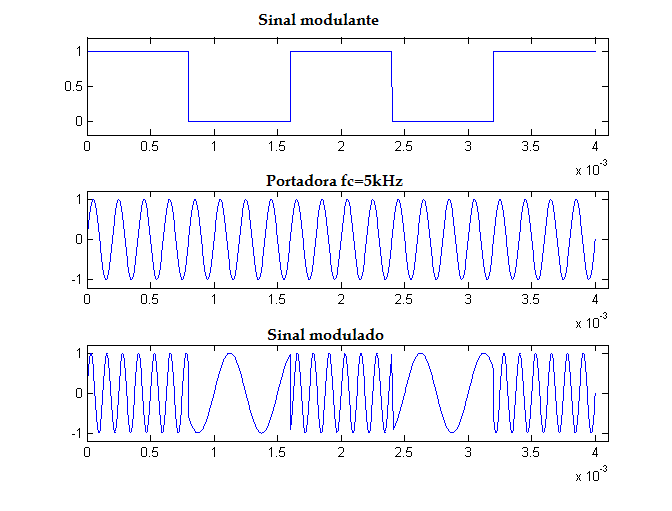
\includegraphics[scale=0.9]{fsk.png}
%    \caption{Modulação FSK}
%    \label{fig:mdfsk}
%\end{figure}
%
%A Figura \ref{fig:mdfsk} mostra um sinal modulante, uma portadora $f_c=5kHz$ com $f_d = 3kHz$.
%É possível observar um sinal em $8kHz$ quando o sinal modulante é "1" e em $2kHz$ quando o sinal modulante é "0", ou seja, o esquema FSK se utiliza da frequência como um meio de transportar a informação, sendo que, para cada frequência $f_i$, é mapeado um simbolo $s_i$.
%
%A largura de banda utilizada na transmissão de sinais modulados em FSK é:
%\[
%BW = 2\cdot \Delta f +2B.
%\]
%
%Onde $BW$ é a largura de banda ocupada, $\Delta f$ é a variação de frequência para representar os bits e $B$ é a banda ocupada desde  $f_c + \Delta f$ até o primeiro nódulo da onda \textit{sinc}, a qual representa o espectro de um nível do sinal. 
%Esse fato fica evidente ao analisarmos a figura \ref{fig:bw}, a qual mostra o espectro de um sinal FSK.
%
%\begin{figure}[H]
%    \centering
%    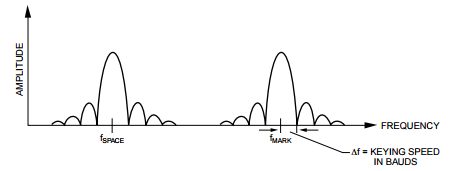
\includegraphics[scale=0.9]{bw}
%    \caption{Espectro de uma sinal modulado com FSK.}
%    \label{fig:bw}
%\end{figure}
%
%\subsubsection{FSK M-ário}
%Para o FSK M-ário, a diferença é que cada símbolos é representado por uma frequência diferente. A largura de banda mínima torna-se:
%
%\[
%BW = M\cdot \Delta f +2B.
%\]
%
%\subsection{Modulação PSK}
%
%O A técnica de modulação conhecida por PSK (Phase Shift- Keying), é o processo pelo qual se altera a fase da onda portadora em função do sinal digital a ser transmitido. Para este processo são usados pulsos bipolares de altura $A_1 = 2$ e $A_0 = -2$ no sinal senoidal da onda portadora em lugar de dois pulsos de altura 0 e A.
%
%Quando ocorrer uma transição de nível lógico do sinal digital a ser transmitido (sinal modulante), haverá uma mudança de 180 graus na fase da onda portadora com relação ao ângulo anterior. A transição observada pode ser tanto de nível lógico "0" para "1" como de nível lógico "1" para "0", como pode ser observado na figura \ref{fig:mpsk}. 
%
%\begin{figure}[H]
%    \centering
%    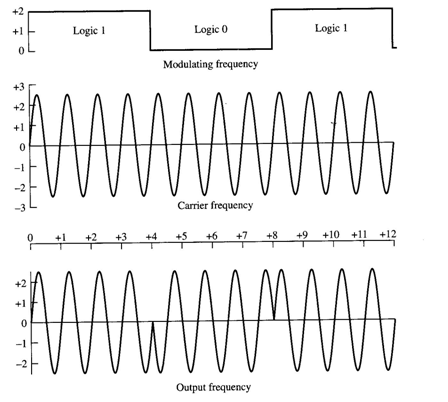
\includegraphics[scale=0.5]{mpsk}
%    \caption{Modulação PSK.}
%    \label{fig:mpsk}
%\end{figure}
%
%Para este tipo de modulação deve se usar a detecção síncrona, já que esta tem como base o conhecimento preciso a respeito da fase da onda portadora recebida, bem como da sua frequência.
%Esta técnica de modulação devido ao fato mencionado, envolve circuitos de recepção (demodulação) mais sofisticados; em compensação oferece melhor desempenho que as técnicas ASK e FSK.